% !TeX program = xelatex
\documentclass[11pt,a4paper,oneside]{article}

\usepackage[margin=2.35cm,headheight=15pt]{geometry}
\usepackage[T1]{fontenc}
\usepackage{lmodern}
\usepackage{amsmath,amssymb}
\usepackage{booktabs,longtable,array}
\usepackage{enumitem}
\usepackage{caption}
\usepackage{float}
\usepackage{xcolor}
\usepackage{microtype}
\usepackage{fancyhdr}
\usepackage[hidelinks]{hyperref}
\usepackage{listings}
\usepackage{tikz}
\usepackage{pgfplots}

\usetikzlibrary{arrows.meta,positioning}
\pgfplotsset{compat=1.18}

\hypersetup{
  colorlinks=true,
  linkcolor=black,
  citecolor=black,
  urlcolor=blue,
  pdftitle={Recover the Design},
  pdfsubject={Degree-constrained exact search with conflict-aware propagation and MRV},
  pdfauthor={}
}

\definecolor{navy}{HTML}{244E6A}
\definecolor{teal}{HTML}{2A7F62}
\definecolor{orange}{HTML}{D27A2C}
\definecolor{rose}{HTML}{A64B5D}
\definecolor{pale}{HTML}{F3F5F7}

\pagestyle{fancy}
\fancyhf{}
\fancyhead[L]{\small Recover the Design}
\fancyhead[R]{\small Anonymous peer review \quad \thepage}
\renewcommand{\headrulewidth}{0.3pt}
\setlength{\parindent}{2em}
\setlength{\parskip}{0.22em}
\renewcommand{\arraystretch}{1.15}
\setlist{itemsep=0.15em,topsep=0.3em}
\captionsetup{font=small,labelfont=bf}

\lstset{
  basicstyle=\ttfamily\small,
  breaklines=true,
  columns=fullflexible,
  frame=lines,
  numbers=left,
  numberstyle=\tiny,
  captionpos=b
}

\title{}
\author{}
\date{}

\begin{document}

\begin{titlepage}
  \centering
  \vspace*{3.2cm}
  {\Huge\bfseries Recover the Design\par}
  \vspace{0.8cm}
  {\Large Degree-Constrained Exact Search with\\[0.2em]
  Event-Driven Propagation and MRV\par}
  \vfill
  {\large Anonymous Peer Review Version\par}
  \vspace{0.5cm}
  {\large 2026-11-03\par}
  \vspace*{2cm}
\end{titlepage}

\pagenumbering{roman}
\begin{abstract}
This project reconstructs an unknown fence design from the degrees of connector
positions. Fences are straight horizontal or vertical segments and may pass
through empty cells. Two perpendicular fences may cross only when the crossing
position contains a connector. The main difficulty is not merely satisfying
vertex degrees: every selected long segment also consumes availability at every
empty cell it crosses.

We model each possible fence as a binary edge between consecutive non-zero
connectors in one row or column. The resulting problem is a degree-constrained
selection problem with pairwise conflict constraints. The exact solver combines
static infeasibility checks, event-driven forcing, immediate conflict rejection,
rollback, and minimum-remaining-values (MRV) branching. A separate validator
reconstructs degrees, endpoint agreement, row ordering, and crossings from the
final text output.

Correctness was checked by exhaustive small-grid enumeration, randomized
differential tests, planted-feasible layouts, and targeted geometric cases. The
24-case Release benchmark uses five measured runs per input. Every case completed
within the 30-second safety timeout; the largest median was 332.151 ms.
Conflict propagation reduced the largest planted search from 39,888 to 162 nodes,
while MRV helped medium inputs but did not improve every case.
\end{abstract}

\noindent\textbf{Keywords:} layout recovery; degree constraints; candidate graph;
event-driven propagation; MRV; exact search; algorithm validation

\setcounter{tocdepth}{1}
\clearpage
\tableofcontents
\clearpage
\pagenumbering{arabic}

\section{Introduction}

\subsection{Problem description}

The input is an $n\times m$ rectangular grid of unit-square positions. A positive
value $k\in\{1,2,3,4\}$ denotes a connector that must be incident to exactly $k$
fence segments. A zero denotes an empty position. Fences are horizontal or
vertical and may be longer than one unit: they may pass through empty positions.
Fences cannot bend, and horizontal and vertical fences may cross only at a
connector.

For each connector, the program outputs its row, column, and four binary states:
up, down, left, and right. If no design exists, the output is
\texttt{No Solution}. The answer is not unique, so the objective is to find any
valid design or to prove that none exists.

\subsection{Key modelling observation}

An initial simplification might connect only adjacent non-zero cells. Sample 3
shows why this is insufficient: a connector in row 1, column 3 connects to a
connector in row 1, column 5, while row 1, column 4 is empty. Thus a candidate
fence must be a maximal straight segment between consecutive non-zero
connectors in one row or one column.

\begin{figure}[H]
\centering
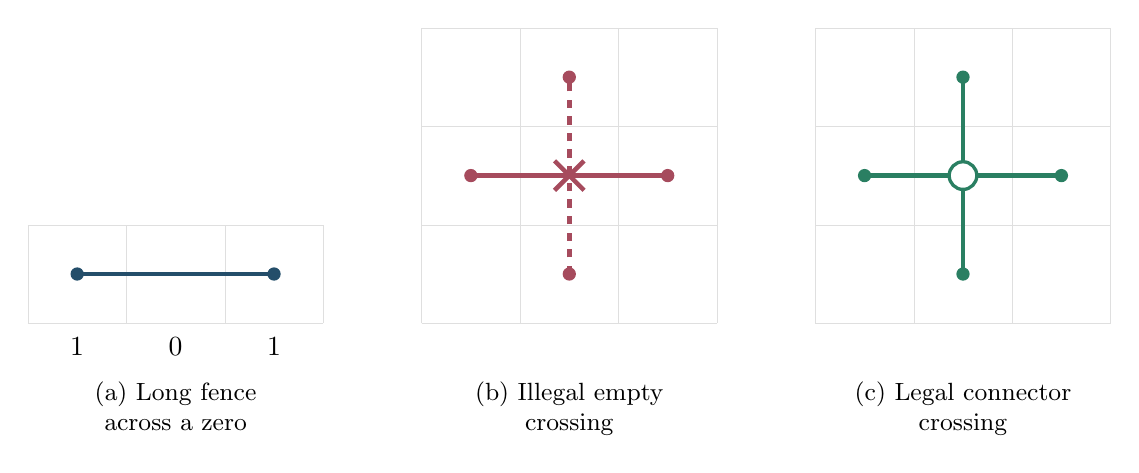
\begin{tikzpicture}[x=1.25cm,y=1.25cm,>=Latex]
  \begin{scope}
    \draw[step=1,gray!25,very thin] (0,0) grid (3,1);
    \fill[navy] (0.5,0.5) circle (2.4pt);
    \fill[navy] (2.5,0.5) circle (2.4pt);
    \draw[ultra thick,navy] (0.5,0.5)--(2.5,0.5);
    \node[below] at (0.5,-0.05) {$1$};
    \node[below] at (1.5,-0.05) {$0$};
    \node[below] at (2.5,-0.05) {$1$};
    \node[below=0.18cm,align=center,font=\small] at (1.5,-0.35)
      {(a) Long fence\\across a zero};
  \end{scope}

  \begin{scope}[xshift=5.0cm]
    \draw[step=1,gray!25,very thin] (0,0) grid (3,3);
    \fill[rose] (0.5,1.5) circle (2.4pt);
    \fill[rose] (2.5,1.5) circle (2.4pt);
    \fill[rose] (1.5,0.5) circle (2.4pt);
    \fill[rose] (1.5,2.5) circle (2.4pt);
    \draw[ultra thick,rose] (0.5,1.5)--(2.5,1.5);
    \draw[ultra thick,rose,dashed] (1.5,0.5)--(1.5,2.5);
    \draw[rose,ultra thick] (1.35,1.35)--(1.65,1.65);
    \draw[rose,ultra thick] (1.35,1.65)--(1.65,1.35);
    \node[below=0.18cm,align=center,font=\small] at (1.5,-0.35)
      {(b) Illegal empty\\crossing};
  \end{scope}

  \begin{scope}[xshift=10cm]
    \draw[step=1,gray!25,very thin] (0,0) grid (3,3);
    \draw[ultra thick,teal] (0.5,1.5)--(2.5,1.5);
    \draw[ultra thick,teal] (1.5,0.5)--(1.5,2.5);
    \fill[white] (1.5,1.5) circle (5pt);
    \draw[teal,very thick] (1.5,1.5) circle (5pt);
    \fill[teal] (0.5,1.5) circle (2.4pt);
    \fill[teal] (2.5,1.5) circle (2.4pt);
    \fill[teal] (1.5,0.5) circle (2.4pt);
    \fill[teal] (1.5,2.5) circle (2.4pt);
    \node[below=0.18cm,align=center,font=\small] at (1.5,-0.35)
      {(c) Legal connector\\crossing};
  \end{scope}
\end{tikzpicture}
\caption{Candidate geometry. A long segment may cross empty cells. Perpendicular
segments form a conflict when they intersect at an empty position, but crossing
at a connector is legal.}
\label{fig:geometry}
\end{figure}

\subsection{Why the problem is not a plain degree matching}

If crossing conflicts were absent, selecting candidate edges to meet prescribed
degrees would be a b-matching relaxation. That relaxation is not a complete
solution. Candidate intervals in a row are disjoint, but a horizontal interval
and a vertical interval can intersect inside a zero cell. Such a pair cannot be
selected simultaneously. The conflict relation therefore introduces a global
0-1 exclusion constraint.

The candidate graph is also not guaranteed to be bipartite. A collinear sequence
of connectors can create odd cycles after gaps are skipped. Consequently, a
simple source-left/right-sink flow construction is not justified by the input
geometry.

\subsection{Contributions}

This implementation contributes:
\begin{itemize}
  \item a long-segment candidate graph that spans arbitrary empty gaps;
  \item a symmetric conflict graph built by scanning empty cells;
  \item an event queue that propagates forced local decisions to fixed point;
  \item immediate crossing rejection and rollback with state trails;
  \item MRV branching on the number of local degree-completion combinations;
  \item an independent validator and a deterministic correctness/performance suite.
\end{itemize}

\section{Data Structure and Algorithm Specification}

\subsection{Notation and candidate graph}

Let $V$ be the set of non-zero connectors and $E$ the set of candidate fence
segments. In each row, sort the non-zero columns and add one candidate between
each consecutive pair. Perform the symmetric construction in each column. For a
connector $v$, let $E_v\subseteq E$ be its incident candidates. The geometry
ensures $|E_v|\le4$.

Each candidate stores its two endpoint vertex ids, the direction from each
endpoint toward the other, and the original endpoint coordinates. A candidate is
horizontal if its endpoint rows are equal.

\subsection{Conflict graph}

For each pair of a horizontal candidate $e$ and a vertical candidate $f$, insert
a symmetric conflict edge when the two segments intersect strictly inside both
open intervals. An equivalent scan visits every empty grid cell and stores at
most one horizontal and one vertical candidate there. Since non-overlapping
candidate intervals partition each row and column, one empty cell yields at most
one conflict pair. The total number of conflict pairs is therefore $O(nm)$.

\subsection{Exact constraints}

Let $x_e\in\{0,1\}$ indicate whether candidate $e$ is selected and $d_v$ be the
required degree of connector $v$. Then
\begin{align}
  \sum_{e\in E_v} x_e &= d_v &&\forall v\in V,\\
  x_e+x_f &\le1 &&\forall(e,f)\in C,
\end{align}
where $C$ is the conflict set. Every selected segment contributes one degree at
each endpoint, so exactly $\frac12\sum_v d_v$ candidate edges must be selected.

\subsection{Static feasibility checks}

Before search the model rejects:
\begin{itemize}
  \item an odd total degree;
  \item a connector whose required degree exceeds its number of candidate edges;
  \item a candidate component with odd degree demand or too few candidate edges.
\end{itemize}
These are necessary conditions. Passing them only means that search is worth
starting.

\subsection{Event-driven propagation}

Each candidate edge has one of three states: \textsc{Unknown},
\textsc{Selected}, or \textsc{Rejected}. For connector $v$, the solver maintains
$s_v$, the number of selected incident edges, and $u_v$, the number of unknown
incident edges. An edge-state change updates its two endpoints and appends both
connectors to an event queue.

For a queued connector with required degree $d_v$:
\begin{itemize}
  \item fail if $s_v>d_v$ or $s_v+u_v<d_v$;
  \item if $s_v=d_v$, reject every unknown incident edge;
  \item if $s_v+u_v=d_v$, select every unknown incident edge.
\end{itemize}
Selecting an edge immediately rejects all of its crossing candidates. Rejections
enqueue their endpoints, so propagation continues to a fixed point.

The queue stores connector ids, not edges or assignments. The implementation
uses a vector and a moving head to avoid repeated deque relocation. Duplicate
events are harmless because each event rereads the current counters.

\begin{lstlisting}[caption={Forced propagation at one connector}]
while pending_head < queue_size:
    v = queue[pending_head++]
    if selected[v] > required[v]: return false
    if selected[v] + unknown[v] < required[v]: return false

    if selected[v] == required[v]:
        reject_all_unknown_edges(v)
    else if selected[v] + unknown[v] == required[v]:
        select_all_unknown_edges(v)
\end{lstlisting}

\subsection{MRV branching}

After propagation, an unsatisfied connector needs
\[
  \mathit{need}_v=d_v-s_v
\]
additional edges. If it has $u_v$ unknown candidates, the number of immediate
local assignments is
\[
  B_v=\binom{u_v}{\mathit{need}_v}.
\]
Because $u_v\le4$, $B_v\le6$. MRV selects the connector with minimum $B_v$.
Ties prefer larger conflict incidence and then the smaller vertex id.

MRV is a variable-ordering heuristic. It does not restrict the allowed values,
so every legal completion remains reachable.

\subsection{DFS, rollback, and completeness}

The search first propagates, then checks whether every connector has exact
degree. Otherwise it enumerates every $\mathit{need}_v$-subset of unknown
incident edges for the MRV connector. Selected edges are committed and the other
incident unknown edges are rejected.

Every state transition records its edge id and previous state in a trail. Failure
rolls back to the branch checkpoint, restores both degree counters, and tries the
next subset. Completeness follows because any valid completion must choose one
of the enumerated local subsets.

\begin{figure}[H]
\centering
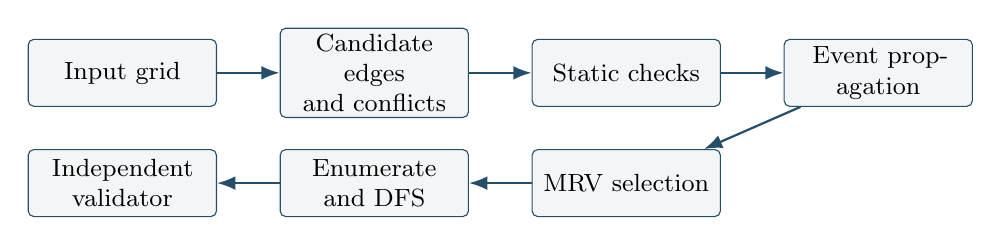
\begin{tikzpicture}[
  box/.style={draw=navy,rounded corners=2pt,fill=pale,align=center,
    text width=2.25cm,minimum height=0.85cm,inner sep=2pt,font=\small},
  arrow/.style={-Latex,thick,navy}
]
  \node[box] (input) at (0,0) {Input grid};
  \node[box] (model) at (3.2,0) {Candidate edges\\and conflicts};
  \node[box] (static) at (6.4,0) {Static checks};
  \node[box] (prop) at (9.6,0) {Event propagation};
  \node[box] (mrv) at (6.4,-1.4) {MRV selection};
  \node[box] (dfs) at (3.2,-1.4) {Enumerate and DFS};
  \node[box] (valid) at (0,-1.4) {Independent validator};

  \draw[arrow] (input)--(model);
  \draw[arrow] (model)--(static);
  \draw[arrow] (static)--(prop);
  \draw[arrow] (prop)--(mrv);
  \draw[arrow] (mrv)--(dfs);
  \draw[arrow] (dfs)--(valid);
\end{tikzpicture}
\caption{Exact solving pipeline. Propagation reaches a local fixed point before
MRV chooses the next connector. A failed branch restores all edge states and
counters through the trail.}
\label{fig:pipeline}
\end{figure}

\subsection{Correctness argument}

Propagation only derives facts that are necessary in every completion. If a
connector has already reached its degree, another selected incident edge would
violate it; if all remaining edges are required to reach the degree, none can be
rejected. A selected edge excludes every crossing candidate by the problem rule.

At a branching node, every completion must choose exactly $\mathit{need}_v$
edges from the connector's unknown candidates. The DFS enumerates every such
subset. Therefore no valid completion is skipped. If all descendants fail, the
current node has no solution. Returning on the first success is valid because
the problem accepts any solution.

\section{Testing Results}

\subsection{Environment and methodology}

\begin{table}[H]
\centering
\caption{Experimental environment}
\begin{tabular}{ll}
\toprule
Item & Configuration \\
\midrule
Platform & Windows, Intel CPU \\
Compiler & MSVC 19.51, Release for benchmarks \\
Build & CMake with Visual Studio 18 2026 generator \\
Correctness & Debug and Release CTest \\
Benchmark repetitions & one warm-up and five measured runs \\
Randomness & deterministic generator seeds \\
\bottomrule
\end{tabular}
\end{table}

Correctness uses two independent existence oracles: the formal solver and a
small-instance edge-subset enumerator. Found layouts are serialized through the
production IO path and checked by the independent validator. The validator
recomputes row-major coverage, degree counts, endpoint agreement, and
empty-cell crossings.

Testing is organized as two complementary layers. White-box C++ groups exercise
parsing, candidate-model invariants, Validator branches, exhaustive differential
enumeration, planted witnesses, propagation counters, and geometric boundaries.
Black-box CLI tests invoke the submitted executable through standard input,
standard output, exit codes, diagnostic modes, and stderr. Every CTest name
identifies one group, so a failure immediately localizes the affected layer
instead of reducing the entire suite to a single pass/fail signal.

\subsection{Correctness coverage}

\begin{figure}[H]
\centering
\begin{tikzpicture}
\begin{axis}[
  xbar,
  xmode=log,
  y dir=reverse,
  width=0.88\linewidth,
  height=10.6cm,
  symbolic y coords={Official samples,Parser cases,Model checks,Validator accepts,Validator rejects,CLI black box,Exhaustive 2x2,Exhaustive 2x3,Random 2x2-3x4,Random 3x3-3x4,Planted feasible,Propagation fixtures,Required geometry},
  ytick=data,
  y tick label style={font=\scriptsize},
  xlabel={Number of test cases (log scale)},
  nodes near coords,
  nodes near coords align={horizontal},
  point meta=explicit symbolic,
  enlarge x limits={0.12,0.15},
  bar width=8pt,
  axis x line*=bottom,
  axis y line*=left,
]
\addplot[fill=navy,draw=navy!80!black]
  table[x=cases,y=test_group,meta=label,col sep=comma]
  {figures/coverage.csv};
\end{axis}
\end{tikzpicture}
\caption{Correctness coverage by test tier. Black-box CLI and rejection groups
are listed separately from exhaustive and randomized solver checks.}
\label{fig:coverage}
\end{figure}

\begin{scriptsize}
\setlength{\tabcolsep}{3pt}
\begin{longtable}{>{\raggedright\arraybackslash}p{2.2cm}r>{\raggedright\arraybackslash}p{3.0cm}>{\raggedright\arraybackslash}p{2.6cm}>{\raggedright\arraybackslash}p{2.6cm}>{\raggedright\arraybackslash}p{1.8cm}c}
\caption{Correctness test cases and observed outcomes}\\
\toprule
Group & Cases & Purpose & Expected & Observed & Failure diagnosis & Status \\
\midrule
\endfirsthead
\toprule
Group & Cases & Purpose & Expected & Observed & Failure diagnosis & Status \\
\midrule
\endhead
Parsing & 13 & Valid grammar and failure isolation & One success, 12 rejections & All matched & n/a & pass \\
Model & 8 & Candidate graph and static proofs & Invariants and reasons hold & All matched & n/a & pass \\
Validator accepts & 5 & Valid layouts and empty design & Status \texttt{valid} & All matched & n/a & pass \\
Validator rejects & 15 & One malformed property per case & Concrete rejection & All matched & n/a & pass \\
CLI black box & 10 & Solve, validate, diagnostics, errors & Required streams and codes & All matched & n/a & pass \\
Official samples & 3 & Feasible, impossible, non-unique & Accepted result & All matched & n/a & pass \\
Exhaustive $2\times2$ & 625 & Every legal degree matrix & Oracle agreement & All matched & n/a & pass \\
Exhaustive $2\times3$ & 15,625 & Complete small input space & Oracle agreement & All matched & n/a & pass \\
Random $2\times2$--$3\times4$ & 1,000 & Fixed-seed differential & Oracle agreement & All matched & n/a & pass \\
Random $3\times3$--$3\times4$ & 3,000 & Larger differential & Oracle agreement & All matched & n/a & pass \\
Planted feasible & up to 200 & Hidden valid witness & Solver finds a layout & All matched & n/a & pass \\
Propagation & 2 & Forced and conflict decisions & Counters increase & All matched & n/a & pass \\
Required geometry & 9 & Long edges, T, cross, disconnection & Expected feasibility & All matched & n/a & pass \\
\bottomrule
\end{longtable}
\end{scriptsize}

All observed cases pass, so no failure diagnosis is pending. The exhaustive tests
compare existence rather than one output string because multiple valid layouts
may exist. For each solver-produced layout the validator checks all constraints
independently. Input failures are kept separate from valid but infeasible
puzzles, and CLI tests verify that usage and diagnostics never contaminate the
answer on standard output.

The default \texttt{correctness} CTest label runs the nine named C++ groups, ten
CLI cases, and the comment-quality gate when Python is available. The complete
24-case benchmark is registered only when
\texttt{ADS\_PROJ3\_ENABLE\_PERFORMANCE\_TESTS} is enabled and is selected by the
separate \texttt{performance} label. This keeps normal correctness runs fast and
independent of timing noise.

On the evaluation environment, all 20 correctness-labelled CTest entries passed
in both Debug and Release builds. The optional performance entry passed all 24
cases with five deterministic repetitions and no search-metric drift.

\subsection{Benchmark design}

The deterministic corpus contains 24 cases from seed \texttt{20261103}. It
contains sparse and dense random degree matrices, planted feasible layouts,
conflict-heavy grids, fragmented components, and infeasible instances. Sizes
range from $10\times10$ to $50\times50$.

Each case is warmed up once. Five measured runs record search nodes, backtracking,
propagation events, forced decisions, conflict rejections, depth, and wall time.
All structural and search counters are identical across the five repetitions.

\begin{figure}[H]
\centering
\begin{tikzpicture}
\begin{axis}[
  ybar,
  ymin=1,
  ymode=log,
  width=0.94\linewidth,
  height=7.2cm,
  ylabel={Visited search nodes (log scale)},
  symbolic x coords={Planted 10,Planted 25,Planted 50,Conflict 50,Dense 50},
  xtick=data,
  x tick label style={rotate=18,anchor=east},
  legend style={at={(0.5,-0.28)},anchor=north,legend columns=3},
  enlarge x limits=0.12,
  bar width=8pt,
]
\addplot[fill=orange] table[x=case,y=degree_only,col sep=comma]
  {figures/node_comparison.csv};
\addplot[fill=teal] table[x=case,y=degree_conflict,col sep=comma]
  {figures/node_comparison.csv};
\addplot[fill=navy] table[x=case,y=mrv,col sep=comma]
  {figures/node_comparison.csv};
\legend{Degree only, Degree + conflict, MRV}
\end{axis}
\end{tikzpicture}
\caption{Search-node comparison. Conflict propagation is the dominant reduction;
MRV helps the medium planted case but chooses a worse early branch on the largest
planted case. The no-propagation baseline is omitted because four large cases
timed out.}
\label{fig:nodes}
\end{figure}

\begin{figure}[H]
\centering
\begin{tikzpicture}
\begin{axis}[
  xbar,
  xmode=log,
  width=0.86\linewidth,
  height=6.5cm,
  symbolic y coords={Planted 10,Planted 25,Planted 50,Conflict 50,Dense 50},
  ytick=data,
  xlabel={Median runtime in milliseconds (log scale)},
  nodes near coords,
  nodes near coords align={horizontal},
  point meta=explicit symbolic,
  nodes near coords style={font=\scriptsize},
  enlarge y limits=0.12,
  bar width=9pt,
]
\addplot[fill=teal,draw=teal!80!black]
  table[x=median_ms,y=case,meta=label,col sep=comma]
  {figures/runtime_comparison.csv};
\end{axis}
\end{tikzpicture}
\caption{Median Release runtime for representative feasible cases. The dense
all-positive graph is slower because MRV scans all unresolved connectors at each
node, even though its node count is identical to fixed order.}
\label{fig:runtime}
\end{figure}

\begin{figure}[H]
\centering
\begin{tikzpicture}
\begin{axis}[
  ybar,
  ymin=1,
  ymode=log,
  unbounded coords=jump,
  width=0.96\linewidth,
  height=7.1cm,
  ylabel={Trigger count (log scale)},
  symbolic x coords={Planted 10,Planted 25,Planted 50,Conflict 50,Dense 50},
  xtick=data,
  x tick label style={rotate=18,anchor=east},
  legend style={at={(0.5,-0.28)},anchor=north,legend columns=3},
  enlarge x limits=0.12,
  bar width=8pt,
]
\addplot[fill=navy] table[x=case,y=forced_select,col sep=comma]
  {figures/propagation_activity.csv};
\addplot[fill=orange] table[x=case,y=forced_reject,col sep=comma]
  {figures/propagation_activity.csv};
\addplot[fill=rose] table[x=case,y=conflict_reject,col sep=comma]
  {figures/propagation_activity.csv};
\legend{Forced select, Forced reject, Conflict reject}
\end{axis}
\end{tikzpicture}
\caption{Propagation activity. Forced decisions and crossing rejections account
for most of the reduction on planted instances. A zero conflict count is omitted
on the logarithmic axis.}
\label{fig:propagation}
\end{figure}

\subsection{Performance and anomalies}

All 24 benchmark cases complete. The maximum median is 332.151 ms and the maximum
single run is 349.880 ms. No case approaches the 30-second safety limit.

\begin{table}[H]
\centering
\caption{Representative node counts and MRV effect}
\begin{tabular}{lrrrr}
\toprule
Case & Degree only & Degree+conflict & MRV & MRV change \\
\midrule
Planted 10x10 & 21 & 14 & 7 & -50.0\% \\
Planted 25x25 & 176,118 & 6,636 & 137 & -97.9\% \\
Planted 50x50 & 39,888 & 162 & 1,404 & +766.7\% \\
Conflict-heavy 50x50 & 271 & 265 & 205 & -22.6\% \\
Dense all-positive 50x50 & 2,402 & 2,402 & 2,402 & 0.0\% \\
\bottomrule
\end{tabular}
\end{table}

The no-propagation baseline completes 20/24 cases under a five-second comparison
limit. Degree-only propagation completes all 24; conflict propagation further
reduces nodes. MRV is not uniformly beneficial. On the largest planted instance,
the fixed order happens to choose a very effective early path, while MRV's local
minimum-domain choice leads to more total nodes.

This result is useful rather than a failure: it demonstrates that local
heuristics must be evaluated against actual search trees. The dense graph also
shows that MRV's scan over all connectors can dominate runtime even when it
cannot reduce the number of nodes.

\section{Analysis and Comments}

\subsection{Preprocessing complexity}

Let $P$ be the number of connectors and $M$ the number of candidate edges. Here
$P\le nm\le2500$ and $M<5000$. Reading the input and assigning vertex ids costs
$O(nm)$. Building row and column candidates is $O(nm+P)$. Marking each candidate
through its interior cells costs $O(nm+M)$ in total because each row and column
interval is traversed once. The conflict graph has at most one pair per empty
cell, hence $O(nm)$ edges.

\subsection{Propagation complexity}

One connector event examines at most four incident edges. If $W$ edge-state
changes occur on one root-to-leaf path, the corresponding event work is $O(W)$
apart from multiple queued events for the same connector. Each such event is
constant-sized and repeats only after a relevant counter changes.

\subsection{MRV complexity}

The current implementation scans all $P$ connectors to choose a branch variable.
For each unresolved connector it inspects at most four incident edges and
computes a binomial coefficient at most six. One MRV selection is therefore
$O(P)$ with a small constant. This explains why dense cases with few backtracks
can still spend visible time in repeated MRV scans.

\subsection{Search and space complexity}

Let $N$ be the number of visited search nodes and $L$ the cost of one node. Total
search cost is $O(NL)$; the worst-case number of nodes remains exponential. The
algorithm stores one byte or byte-sized state per candidate edge, two counters per
connector, a rollback trail, the queue, candidate endpoints, and conflict
adjacency. All are bounded by $O(nm+M)$.

\subsection{Limitations}

No official time limit is given by the problem statement. Measurements therefore
describe the current machine, compiler, seed set, and chosen corpus. A separate
50 by 50 planted probe with density 0.50--0.55 exceeded a 15--30 second safety
window. This is explicitly excluded from the fixed acceptance corpus and is
reported as a limitation for dense random adversarial degree systems.

The conflict graph captures only forbidden selection pairs. Component
decomposition is not applied directly because conflict edges can couple
candidate graph components that share no connector.

\subsection{Possible improvements}

The most direct improvement is to maintain the set of unresolved connectors and
incrementally track candidate domain sizes instead of rescanning all connectors
for every MRV decision. A second option is one-step lookahead after each local
combination. A third is to decompose conflict-connected components and apply
separate max-flow or b-matching bounds when a component is bipartite.

These changes should be evaluated against the current baseline. The existing
results show that a heuristic can reduce one family of instances while degrading
another, so portfolio selection based on model structure may be more useful than
applying one ordering rule everywhere.

\appendix
\section{Source Code and Reproduction}

\subsection{Source organization}

\begin{table}[H]
\centering
\caption{Main source responsibilities}
\begin{tabular}{ll}
\toprule
File & Responsibility \\
\midrule
\texttt{io.cpp/hpp} & Strict input parsing and row-major output \\
\texttt{model.cpp/hpp} & Connector, candidate and conflict construction \\
\texttt{solver.cpp/hpp} & Propagation, rollback, MRV and DFS \\
\texttt{validator.cpp/hpp} & Independent answer validation \\
\texttt{test\_runner.cpp} & Nine named unit, solver, and Validator groups \\
\texttt{run\_cli\_tests.cmake} & Black-box CLI streams and exit codes \\
\texttt{run\_performance\_tests.cmake} & Optional deterministic corpus CTest \\
\texttt{benchmark\_runner.cpp} & Repetition and CSV instrumentation \\
\bottomrule
\end{tabular}
\end{table}

\subsection{Key source excerpts}

The complete source is in the submission \texttt{code} directory. The following
excerpt shows the two propagation forcing conditions.

\begin{lstlisting}[language=C++,caption={Forced propagation excerpt}]
if (selected == required) {
    // Any additional edge would exceed the target degree.
    for (int edgeId : incidentEdges[v])
        if (state[edgeId] == UNKNOWN)
            assignRejected(edgeId);
} else if (selected + unknown == required) {
    // Every unknown edge is required to reach the target.
    for (int edgeId : incidentEdges[v])
        if (state[edgeId] == UNKNOWN)
            assignSelected(edgeId);
}
\end{lstlisting}

The next excerpt shows the local domain size used by MRV.

\begin{lstlisting}[language=C++,caption={MRV domain size excerpt}]
int need = requiredDegree[v] - selectedDegree[v];
int combinations = 1;
for (int i = 0; i < need; ++i) {
    combinations *= static_cast<int>(available.size()) - i;
    combinations /= i + 1;
}
// Choose the connector with the smallest value of C(available,need).
\end{lstlisting}

\subsection{Build and run}

\begin{lstlisting}[language=bash,caption={Reproduction commands}]
cmake -S . -B build -G "Visual Studio 18 2026" -A x64
cmake --build build --config Release
ctest --test-dir build -C Release -L correctness --output-on-failure
./build/Release/recover.exe < input.txt
\end{lstlisting}

\section{Benchmark Reproduction}

The report figures are rendered by PGFPlots from compact CSV files generated by
\path{tools/prepare_report_data.py}. The full results are generated by:

\begin{lstlisting}[language=bash]
python tools/generate_cases.py --output-dir data/generated
python tools/run_benchmarks.py \
  --benchmark-exe build/Release/recover_benchmark.exe \
  --cases-dir data/generated --output-dir data/experiments \
  --label mrv --repeat 5 --timeout 30
python tools/compare_benchmarks.py
python tools/prepare_report_data.py
\end{lstlisting}

When Python 3 is available, the same 24-case corpus can be run through CTest:

\begin{lstlisting}[language=bash]
cmake -S . -B build -DADS_PROJ3_ENABLE_PERFORMANCE_TESTS=ON
ctest --test-dir build -C Release -L performance --output-on-failure
\end{lstlisting}

Each raw benchmark row contains model size, conflict count, found status, DFS
nodes, backtracks, propagation events, forced select/reject counts, crossing
rejections, maximum depth, and wall time. The aggregation script reports median,
mean, and maximum runtime.

\begin{thebibliography}{9}
\bibitem{russell}
S. Russell and P. Norvig.
\textit{Artificial Intelligence: A Modern Approach}.
Pearson, fourth edition, 2020.

\bibitem{knuth4a}
D. E. Knuth.
\textit{The Art of Computer Programming, Volume 4A: Combinatorial Algorithms}.
Addison-Wesley, 2011.
\end{thebibliography}

\clearpage
\section*{Author List}
\addcontentsline{toc}{section}{Author List}
Author identities and contribution details are withheld in this anonymous peer
review version.

\section*{Declaration}
\addcontentsline{toc}{section}{Declaration}
We hereby declare that all work done in this project is of our independent
effort as a group.

\end{document}
